\begin{figure}[htbp]
\centering
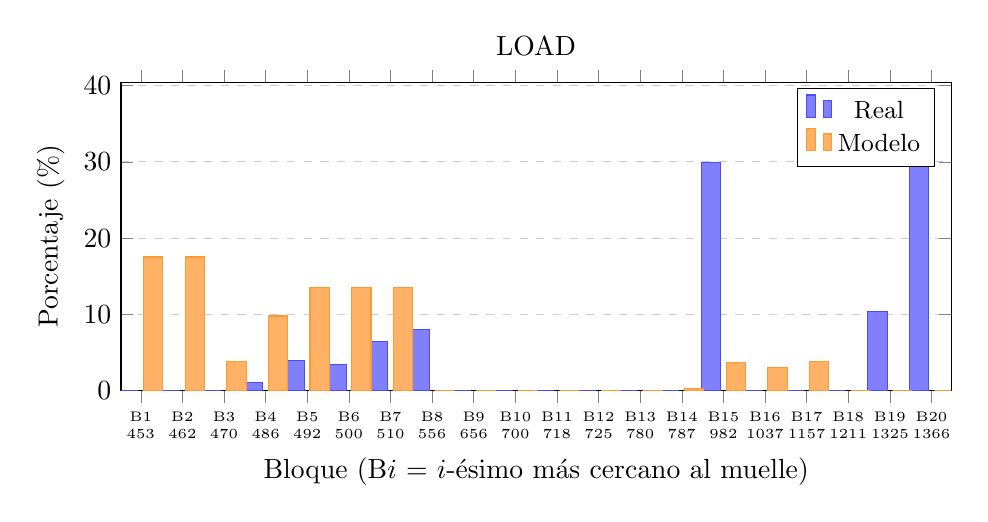
\begin{tikzpicture}
\begin{axis}[
  ybar, bar width=7pt, width=\textwidth, height=5.5cm,
  title={LOAD},
  xlabel={Bloque (B$i$ = $i$-ésimo más cercano al muelle)},
  ylabel={Porcentaje (\%)},
  xtick={0,1,2,3,4,5,6,7,8,9,10,11,12,13,14,15,16,17,18,19},
  xticklabels={{B1\\453},{B2\\462},{B3\\470},{B4\\486},{B5\\492},{B6\\500},{B7\\510},{B8\\556},{B9\\656},{B10\\700},{B11\\718},{B12\\725},{B13\\780},{B14\\787},{B15\\982},{B16\\1037},{B17\\1157},{B18\\1211},{B19\\1325},{B20\\1366}},
  xticklabel style={font=\tiny, align=center},
  ymin=0,
  legend style={at={(0.98,0.98)}, anchor=north east, font=\small},
  ymajorgrids=true, grid style={dashed,gray!40},
  enlarge x limits=0.025,
]
\addplot[fill=blue!50, draw=blue!70] coordinates {(0,0.00) (1,0.00) (2,0.00) (3,1.05) (4,3.95) (5,3.43) (6,6.46) (7,8.04) (8,0.00) (9,0.00) (10,0.00) (11,0.00) (12,0.00) (13,0.00) (14,29.91) (15,0.00) (16,0.00) (17,0.00) (18,10.41) (19,36.76)};
\addplot[fill=orange!60, draw=orange!80] coordinates {(0,17.52) (1,17.52) (2,3.81) (3,9.79) (4,13.49) (5,13.49) (6,13.49) (7,0.00) (8,0.00) (9,0.00) (10,0.00) (11,0.00) (12,0.00) (13,0.33) (14,3.70) (15,3.05) (16,3.81) (17,0.00) (18,0.00) (19,0.00)};
\legend{Real, Modelo}
\end{axis}
\end{tikzpicture}
\vspace{4pt}
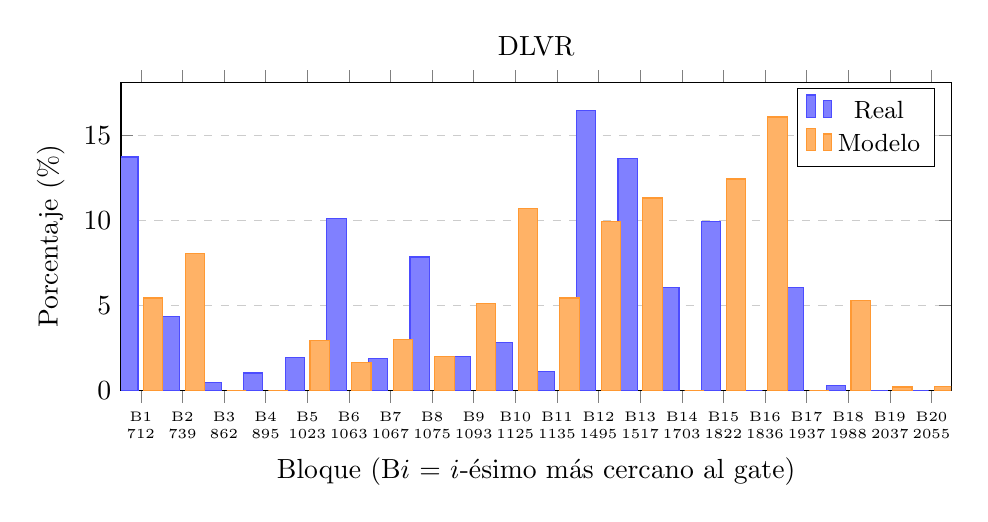
\begin{tikzpicture}
\begin{axis}[
  ybar, bar width=7pt, width=\textwidth, height=5.5cm,
  title={DLVR},
  xlabel={Bloque (B$i$ = $i$-ésimo más cercano al gate)},
  ylabel={Porcentaje (\%)},
  xtick={0,1,2,3,4,5,6,7,8,9,10,11,12,13,14,15,16,17,18,19},
  xticklabels={{B1\\712},{B2\\739},{B3\\862},{B4\\895},{B5\\1023},{B6\\1063},{B7\\1067},{B8\\1075},{B9\\1093},{B10\\1125},{B11\\1135},{B12\\1495},{B13\\1517},{B14\\1703},{B15\\1822},{B16\\1836},{B17\\1937},{B18\\1988},{B19\\2037},{B20\\2055}},
  xticklabel style={font=\tiny, align=center},
  ymin=0,
  legend style={at={(0.98,0.98)}, anchor=north east, font=\small},
  ymajorgrids=true, grid style={dashed,gray!40},
  enlarge x limits=0.025,
]
\addplot[fill=blue!50, draw=blue!70] coordinates {(0,13.74) (1,4.35) (2,0.49) (3,1.04) (4,1.95) (5,10.12) (6,1.91) (7,7.86) (8,2.02) (9,2.85) (10,1.11) (11,16.49) (12,13.67) (13,6.05) (14,9.95) (15,0.00) (16,6.05) (17,0.31) (18,0.03) (19,0.00)};
\addplot[fill=orange!60, draw=orange!80] coordinates {(0,5.45) (1,8.06) (2,0.00) (3,0.00) (4,2.96) (5,1.68) (6,3.02) (7,1.99) (8,5.14) (9,10.71) (10,5.45) (11,9.93) (12,11.33) (13,0.00) (14,12.45) (15,16.09) (16,0.00) (17,5.29) (18,0.22) (19,0.25)};
\legend{Real, Modelo}
\end{axis}
\end{tikzpicture}
\caption{Distribución porcentual de flujos por bloque, semana~12 (2022-03-21). Bloques ordenados por distancia creciente al destino.}
\label{fig:flujos-sem12}
\end{figure}